% !TeX root = ../report.tex

Different from the previous studies, the determining factor of the pressure in this study is how many different bundles of rays pass through a cube, instead of the number of intersected rays. A bundle is determined by origin transducer element, the history of the media and type of the rays (longitudinal or shear). There are many rays in each bundle, but not as many if they are required to pass through the same sampling cube. Although increasing the number of rays still tends to produce a better simulation quality, the relation is no longer simple.

When running in serial, the model is about 2.5 times faster than the old method with the same number of rays. when the ray number is 200, the result is already showing a cigar shaped focus area. The code in this model is also optimized for parallelization. Each transducer can be allocated on one separate process. The parallelization is implemented in python using its \texttt{multiprocessing} library. This study is conducted on a workstation with Intel\text{\textregistered} Xeon\text{\textregistered} CPU E3-1230 v5 3.40GHz. The CPU has 4 cores in total (8 cores if considering virtual CPU), hence, the simulation creates a process pool with 8 workers. In this way, the simulation is approximately 4 time faster than the simulation run in serial. The reason why it is not 8 times faster is probably the data exchanges between processes cost a longer time. The program can be further optimized if the ray-box intersection and sampling is implement on GPU, as the algorithm is almost embarrassingly parallel in that regard.

\begin{figure}[h]
    \centering
    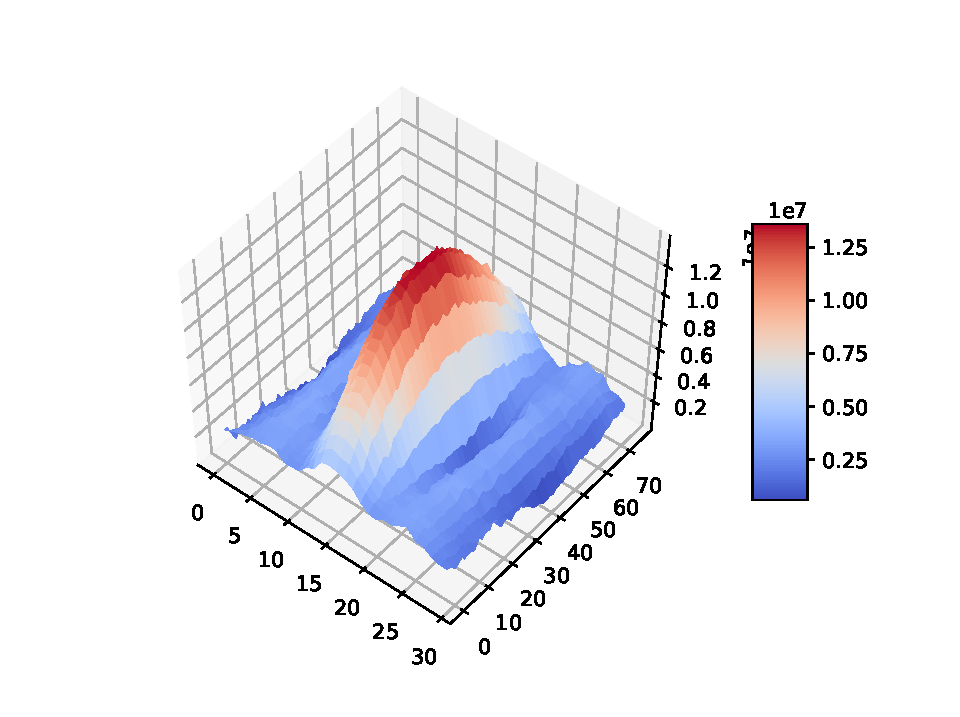
\includegraphics[width=0.6\textwidth]{same_smooth}
    \caption{Result from this study that is closest to gold standard (4500 rays  per transducer element, simulation time 2hrs)}
    \label{fig:same_smooth}
\end{figure}

This study introduces a new way to simulate the propagation of ultrasound ways in HIFU system using beam spreading. The goal of this study was to prove the feasibility of this new method. The model is based on acoustics laws and is capable of handling the interference. The model is tested on a simple geometry. It could be extended to support more complicated geometries. In application, the geometry model usually consists of triangular mesh with plane boundaries, which are compatible with the plane implemented in this study. However, the porous structure of the bone might be a challenge to the model \cite{vanwijk2013} because the reflection and refraction could be more complicated than that in this study. Further research is needed to determine the scaling factor to scale the result in this study to physical value. The pressure can then be converted to temperature in the geometry.
